\section{Results}
\label{sec:chap_slam_results}

For our experiments, we used a \textit{C++} implementation developed by Bastian Steder of the algorithm presented in Section~\ref{sec:chap_slam_algo}. This version of the algorithm provides a score (between 0 and 1) for each pair of scan in the database. It is the responsibility of the user to choose the threshold at which the scans will be considered as coming from the same place or not. The definition of a place can also be variable and we choose to use a threshold on the distance between the centers of scans. 

For each path we did the acquisition twice. The first run to get the first examples and the second run should be recognized places.
\todo{explain the odometry and icp for ground truth here.}

Note that for our experiments we tried both with and without the rotation invariance parameter, but since using it reduced significantly the result in our case, we wont discuss it. 

For a comprehensive graphical representation of scores between each pair of scans, we use confusion matrices. Columns and rows represents ordered scans\dots
The color between black (score = 0) and white (score = 1)

\dots Confusion matrix: The dark areas that are not close to the main diagonal mark loop closures.

\todo{I might want a single figure with the three matrices on the left and the 3 prec recall on the right\dots}\\
\todo{When explaining matrices, notice that each square represent an acquisition, not a distance, and distance between scans is variable\dots therefore prec recall curves\dots it still show if there is obvious error such a white dot in the middle of nowhere}

\begin{figure}[H]
    \centering
    \subfloat[]{\label{fig:result_matrix_structured}}{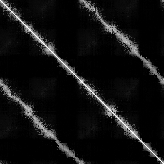
\includegraphics[width=0.40\linewidth]{img/chap_slam/matrix_structured.png}}
    \subfloat[]{\label{fig:result_curve_structured}}{
\includegraphics[width=0.40\linewidth]{img/todo.jpg}} \\
    \subfloat[]{\label{fig:result_matrix_forest}}{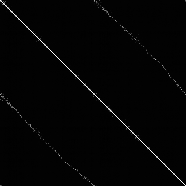
\includegraphics[width=0.40\linewidth]{img/chap_slam/matrix_forest.png}}
    \subfloat[]{\label{fig:result_curve_forest}}{
\includegraphics[width=0.40\linewidth]{img/todo.jpg}} \\
    \subfloat[]{\label{fig:result_matrix_velodyne}}{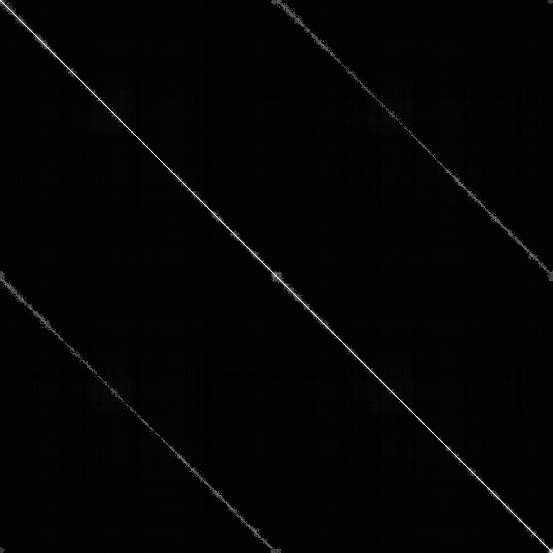
\includegraphics[width=0.40\linewidth]{img/chap_slam/matrix_velodyne.png}}
    \subfloat[]{\label{fig:result_curve_velodyne}}{
\includegraphics[width=0.40\linewidth]{img/todo.jpg}} \\
    \caption[todo]{\protect\subref{fig:result_matrix_structured} is the confusion matrix for both loops of the structured dataset (XX scans) and \protect\subref{fig:result_curve_structured} is the recall curve. \protect\subref{fig:result_matrix_forest} and \protect\subref{fig:result_curve_forest} are the corresponding matrix and recall curve for the unstructured dataset and \protect\subref{fig:result_matrix_forest} and \protect\subref{fig:result_curve_forest} are for the unstructured dataset using the velodyne.}
    \label{fig:chap_slam_results}
\end{figure}

%\begin{figure}[htpb]
    %\centering
    %
\includegraphics[width=0.2\linewidth]{img/todo.jpg}
    %\caption[todo]{Nice to have: matched keypoints (something like an histogram of dist, height or avg dist per scan)}
    %\label{fig:match_avg_dist}
%\end{figure}


\section{Discussion}
\label{sec:chap_slam_discussion}
\todo{I dont know if I want to split in result (purely result) and discussion}
\begin{itemize}
    \item Because distance is smaller on avg in the forest, cause parallax
    \item Also more occlusion, but this also why the env. is complex. As said earlier range img kind of deal with it.
\end{itemize}

\subsection{Structured vs Forest}
\label{ssec:chap_slam_struct_vs_forest}

\subsection{SICK vs Velodyne}
\label{ssec:chap_slam_sick_vs_velodyne}
